\section{Results and discussion}
\label{sec:results}
%************************************************

\subsection{Experiments}
\label{subsec:experiments}

Initially, experimental values identifying the bulk behavior, $\mu_{psh}$, $\mu_{sh}$ and $\rho_{b}$, 
for sinter fine have been acquired through the $SRSCT$. 
The $\mu_{psh}$ was calculated as average of the $\mu_{ie}$ in the first
experimental plateau.
As average of $\mu_{ie}$ in the second plateau we obtained $\mu_{sh}$.
Later, two $AOR$ test have been performed, thus identifying an average angle of
$38.85 ^\circ$.

\subsection{DEM Simulations}
\label{subsec:simulations}

For sinter fine 546 shear cell and 81 static angle of repose simulations have
been realized.
The computational time resulted in 1 hour with 32 AMD cores for a benchmark
shear cell simulation and 9 hours for a benchmark $AOR$ simulation, both with 50K particles. 
Simulations with large $dCylDp$ required a greater time amount (e.g. with 400K
particles about 12 hours for the shear cell).

\subsection{ANN model development}
\label{subsec:annmodeldev}

We processed the random combinations with the $NN$.
We represented the tabbed combinations ($TC1$) for one load condition of the
shear cell ($\sigma_n=10070 ~[Pa]$) in Fig.
\ref{fig:24radarpirker1schulze10070}.
Here, the minimum and maximum values, together with the mean and the confidence
range, provided by the square deviation, are shown. 
Notably, the confidence range is large (dark grey), 
especially for the $COR$, highlighting its scarce influence over the characterization. 
Instead, both the $\rho_p$  and the $\mu_s$ show a narrow confidence range, 
displaying at the same time their influence and the validity of this procedure to find valid $DEM$ parameters. 
That agrees with the examination of the ratio of the standard deviation to the
range.
We then processed the random combinations with the $AOR$ $NN$. 
Finally, we extracted from the $TC1$ values the $AOR$ $NN$ behaviour
and compared it with the experimental one.
As can be seen in the radar plot in Fig.
\ref{fig:33radarpirker1schulze10070aor}, the confidence range is meager, indicating that all the parameters but the $COR$ 
had an important role and the reliability of these parameters combinations to represent the bulk behaviour. 
From the initial 6250000 combinations, only 3884 of them were valid.
% \begin{figure}[htp] \centering
%     \begin{subfig}[width=0.40\columnwidth]{width=0.40\columnwidth}
%         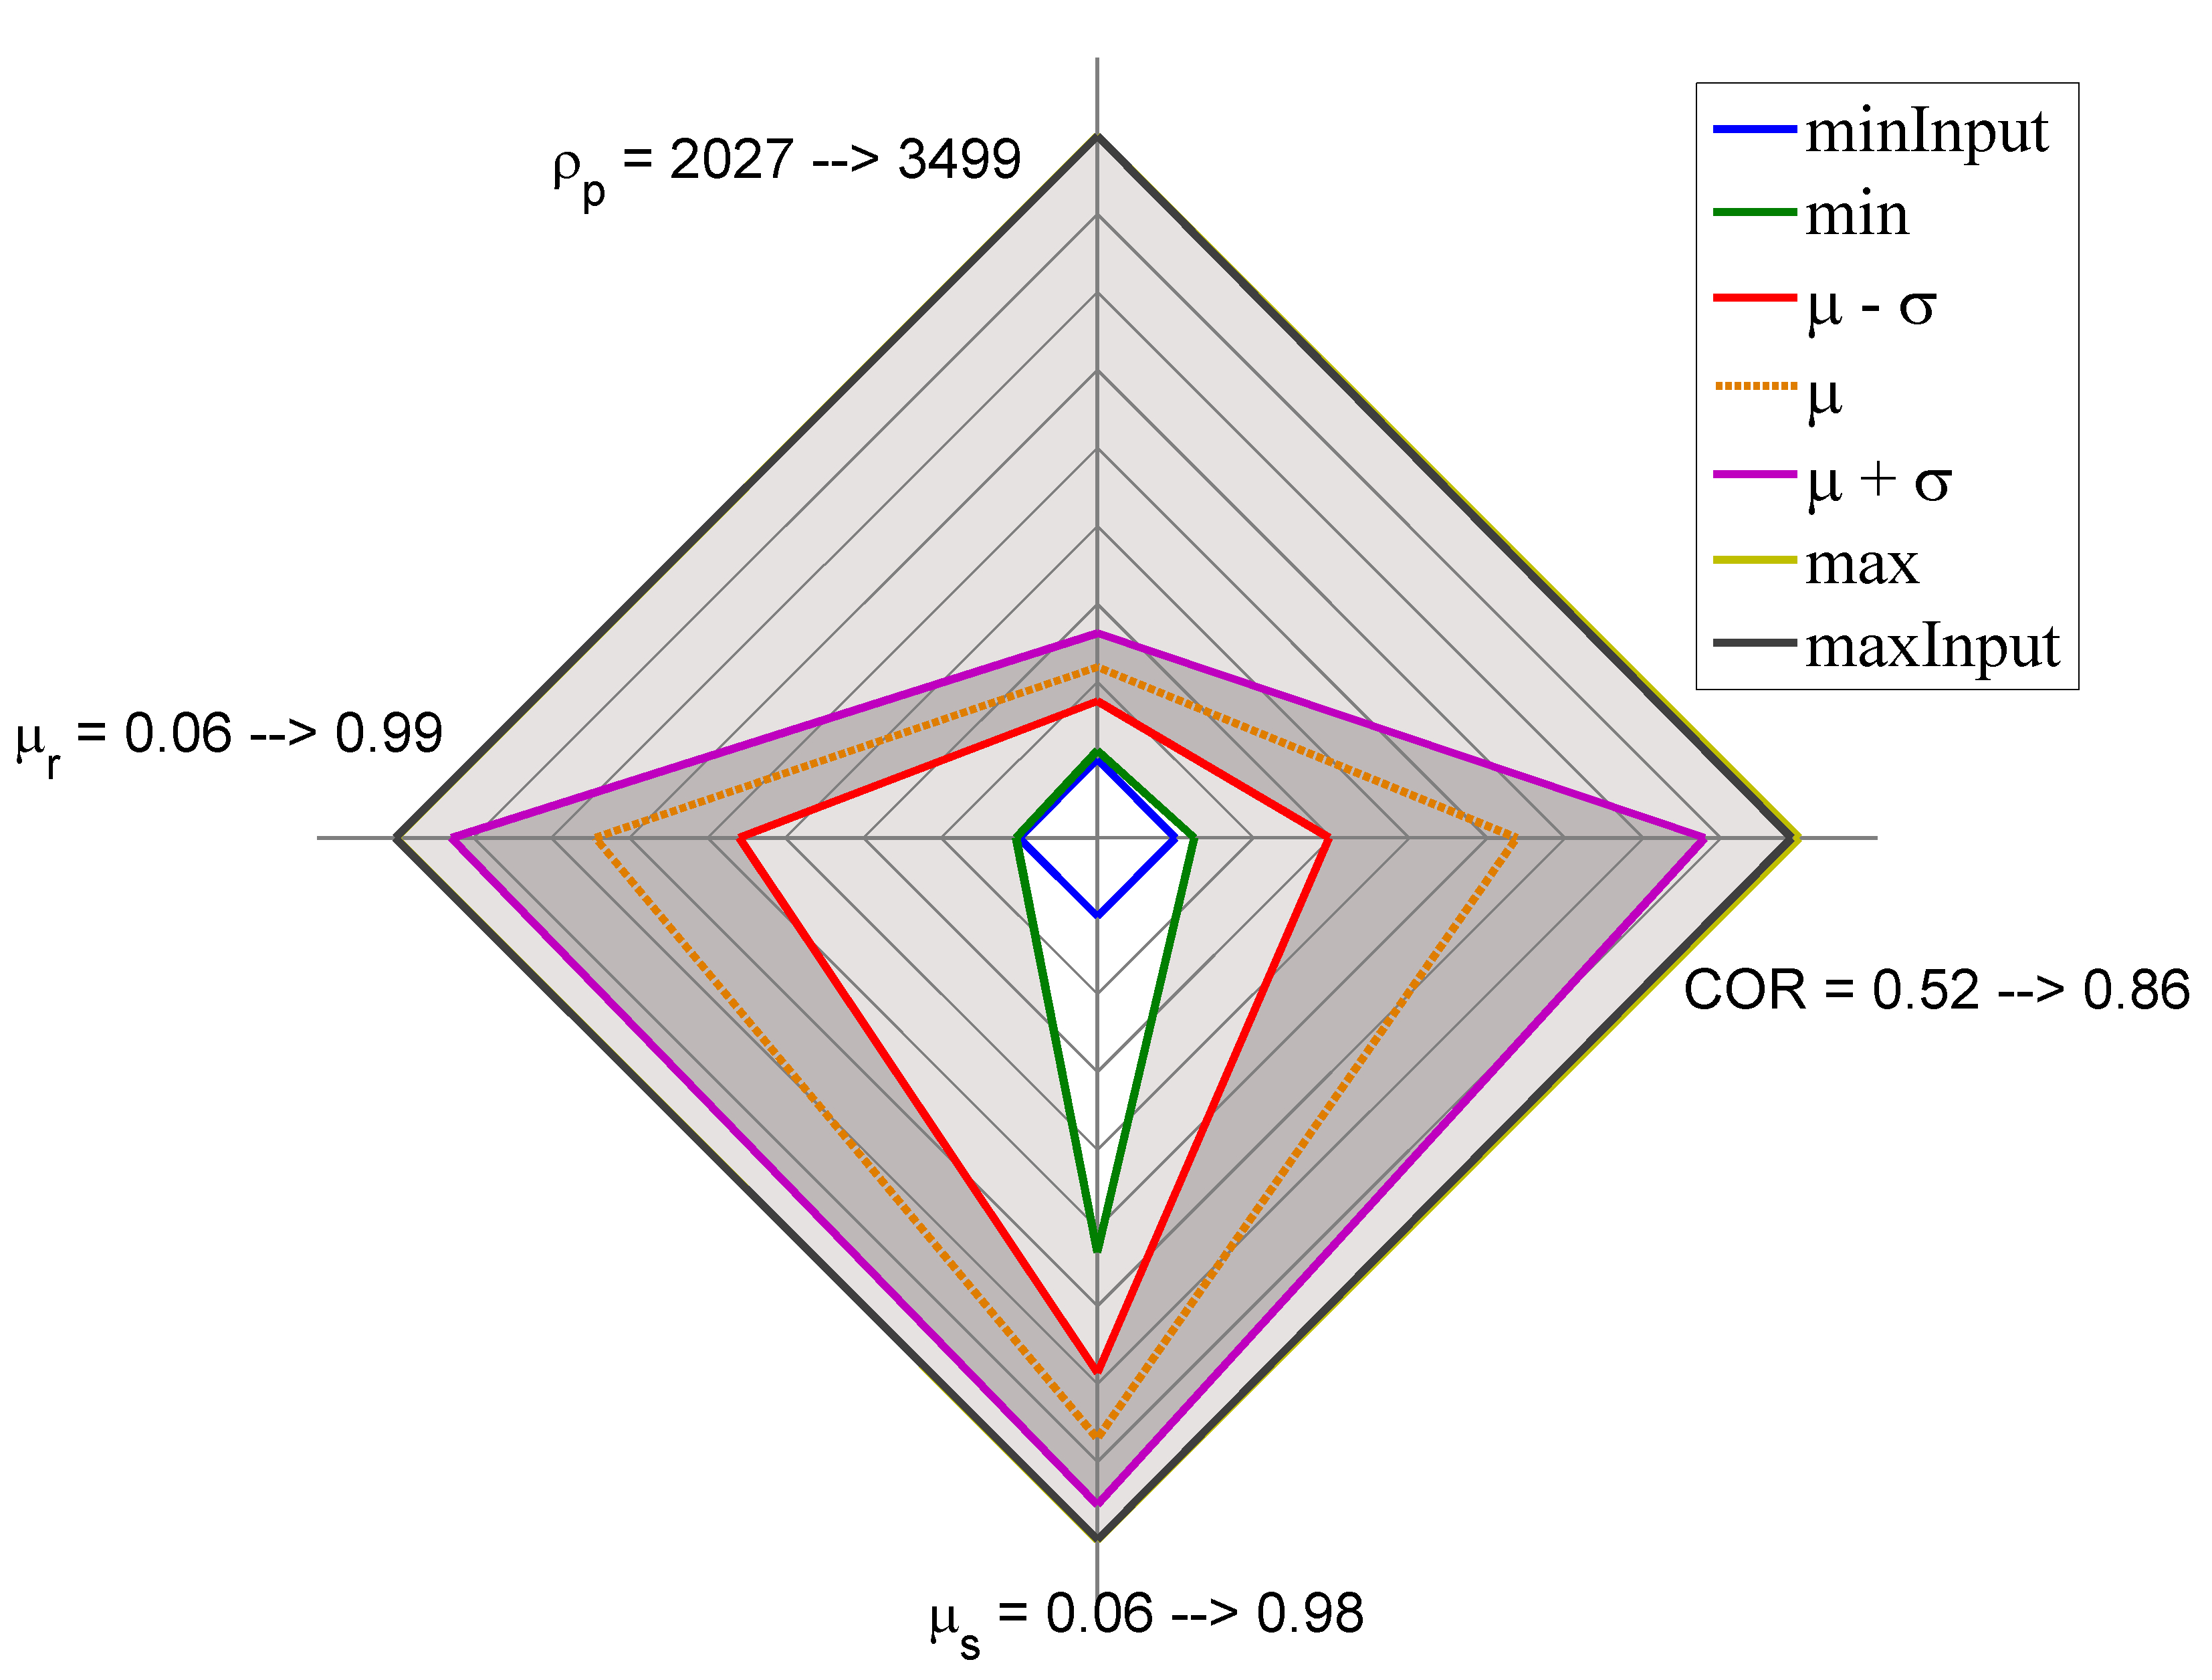
\includegraphics[width=\textwidth]{images/original/24radarpirker1schulze10070}
%         \caption{Cloud plot, $AOR_{exp} = 38.85 ^\circ$}
%         \label{fig:32cloudpirker1aor} 
%     \end{subfig}\ \quad
%     \begin{subfig}[width=0.40\columnwidth]{width=0.40\columnwidth}
%         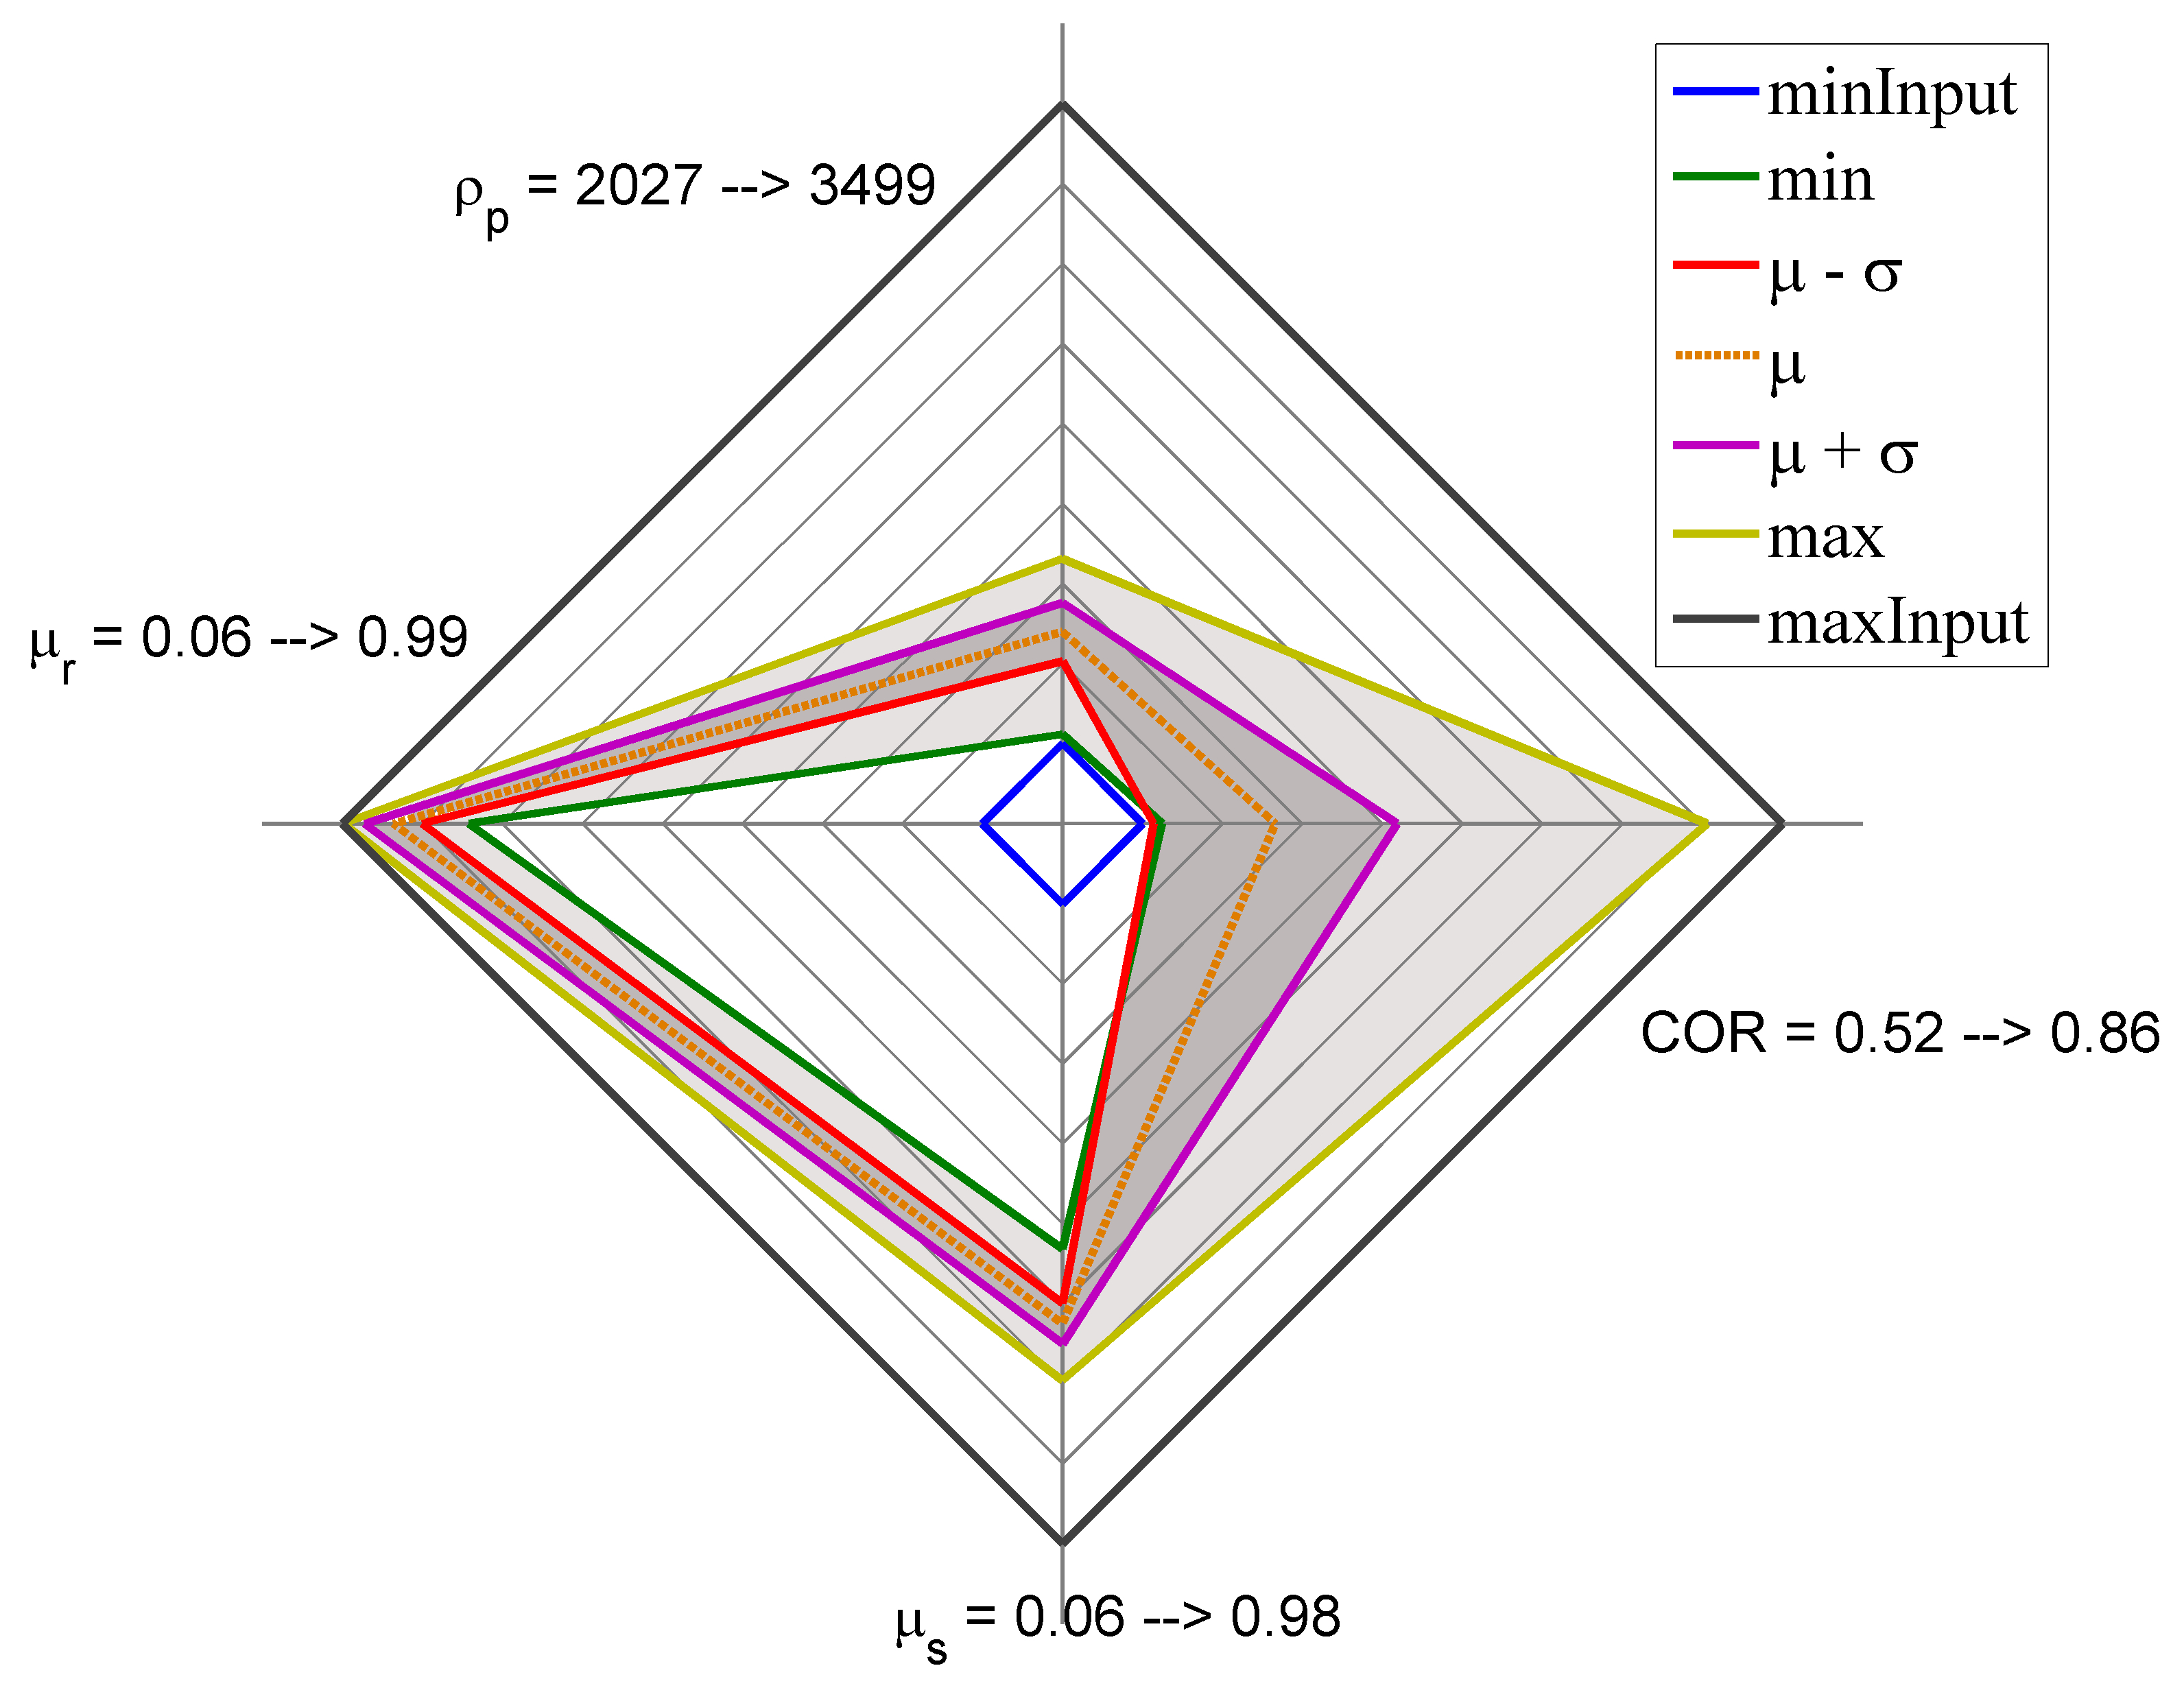
\includegraphics[width=\textwidth]{images/original/33radarpirker1schulze10070aor}
%         \caption{Cloud plot, $AOR_{exp} = 38.85
%         ^\circ$ \& $SCT$: $\sigma_n=10070 ~[Pa]$}
%         \label{fig:34cloudpirker1schulze10070aor} 
%     \end{subfig}
%     \caption{Density plot comparison of AOR and SCT results}
%     \label{fig:35schulze10070aorradarandcloud}
% \end{figure}

\begin{figure}[tb]
\centering
\subfloat[Radar Schulze 10070 Pa]
{\label{fig:24radarpirker1schulze10070}%
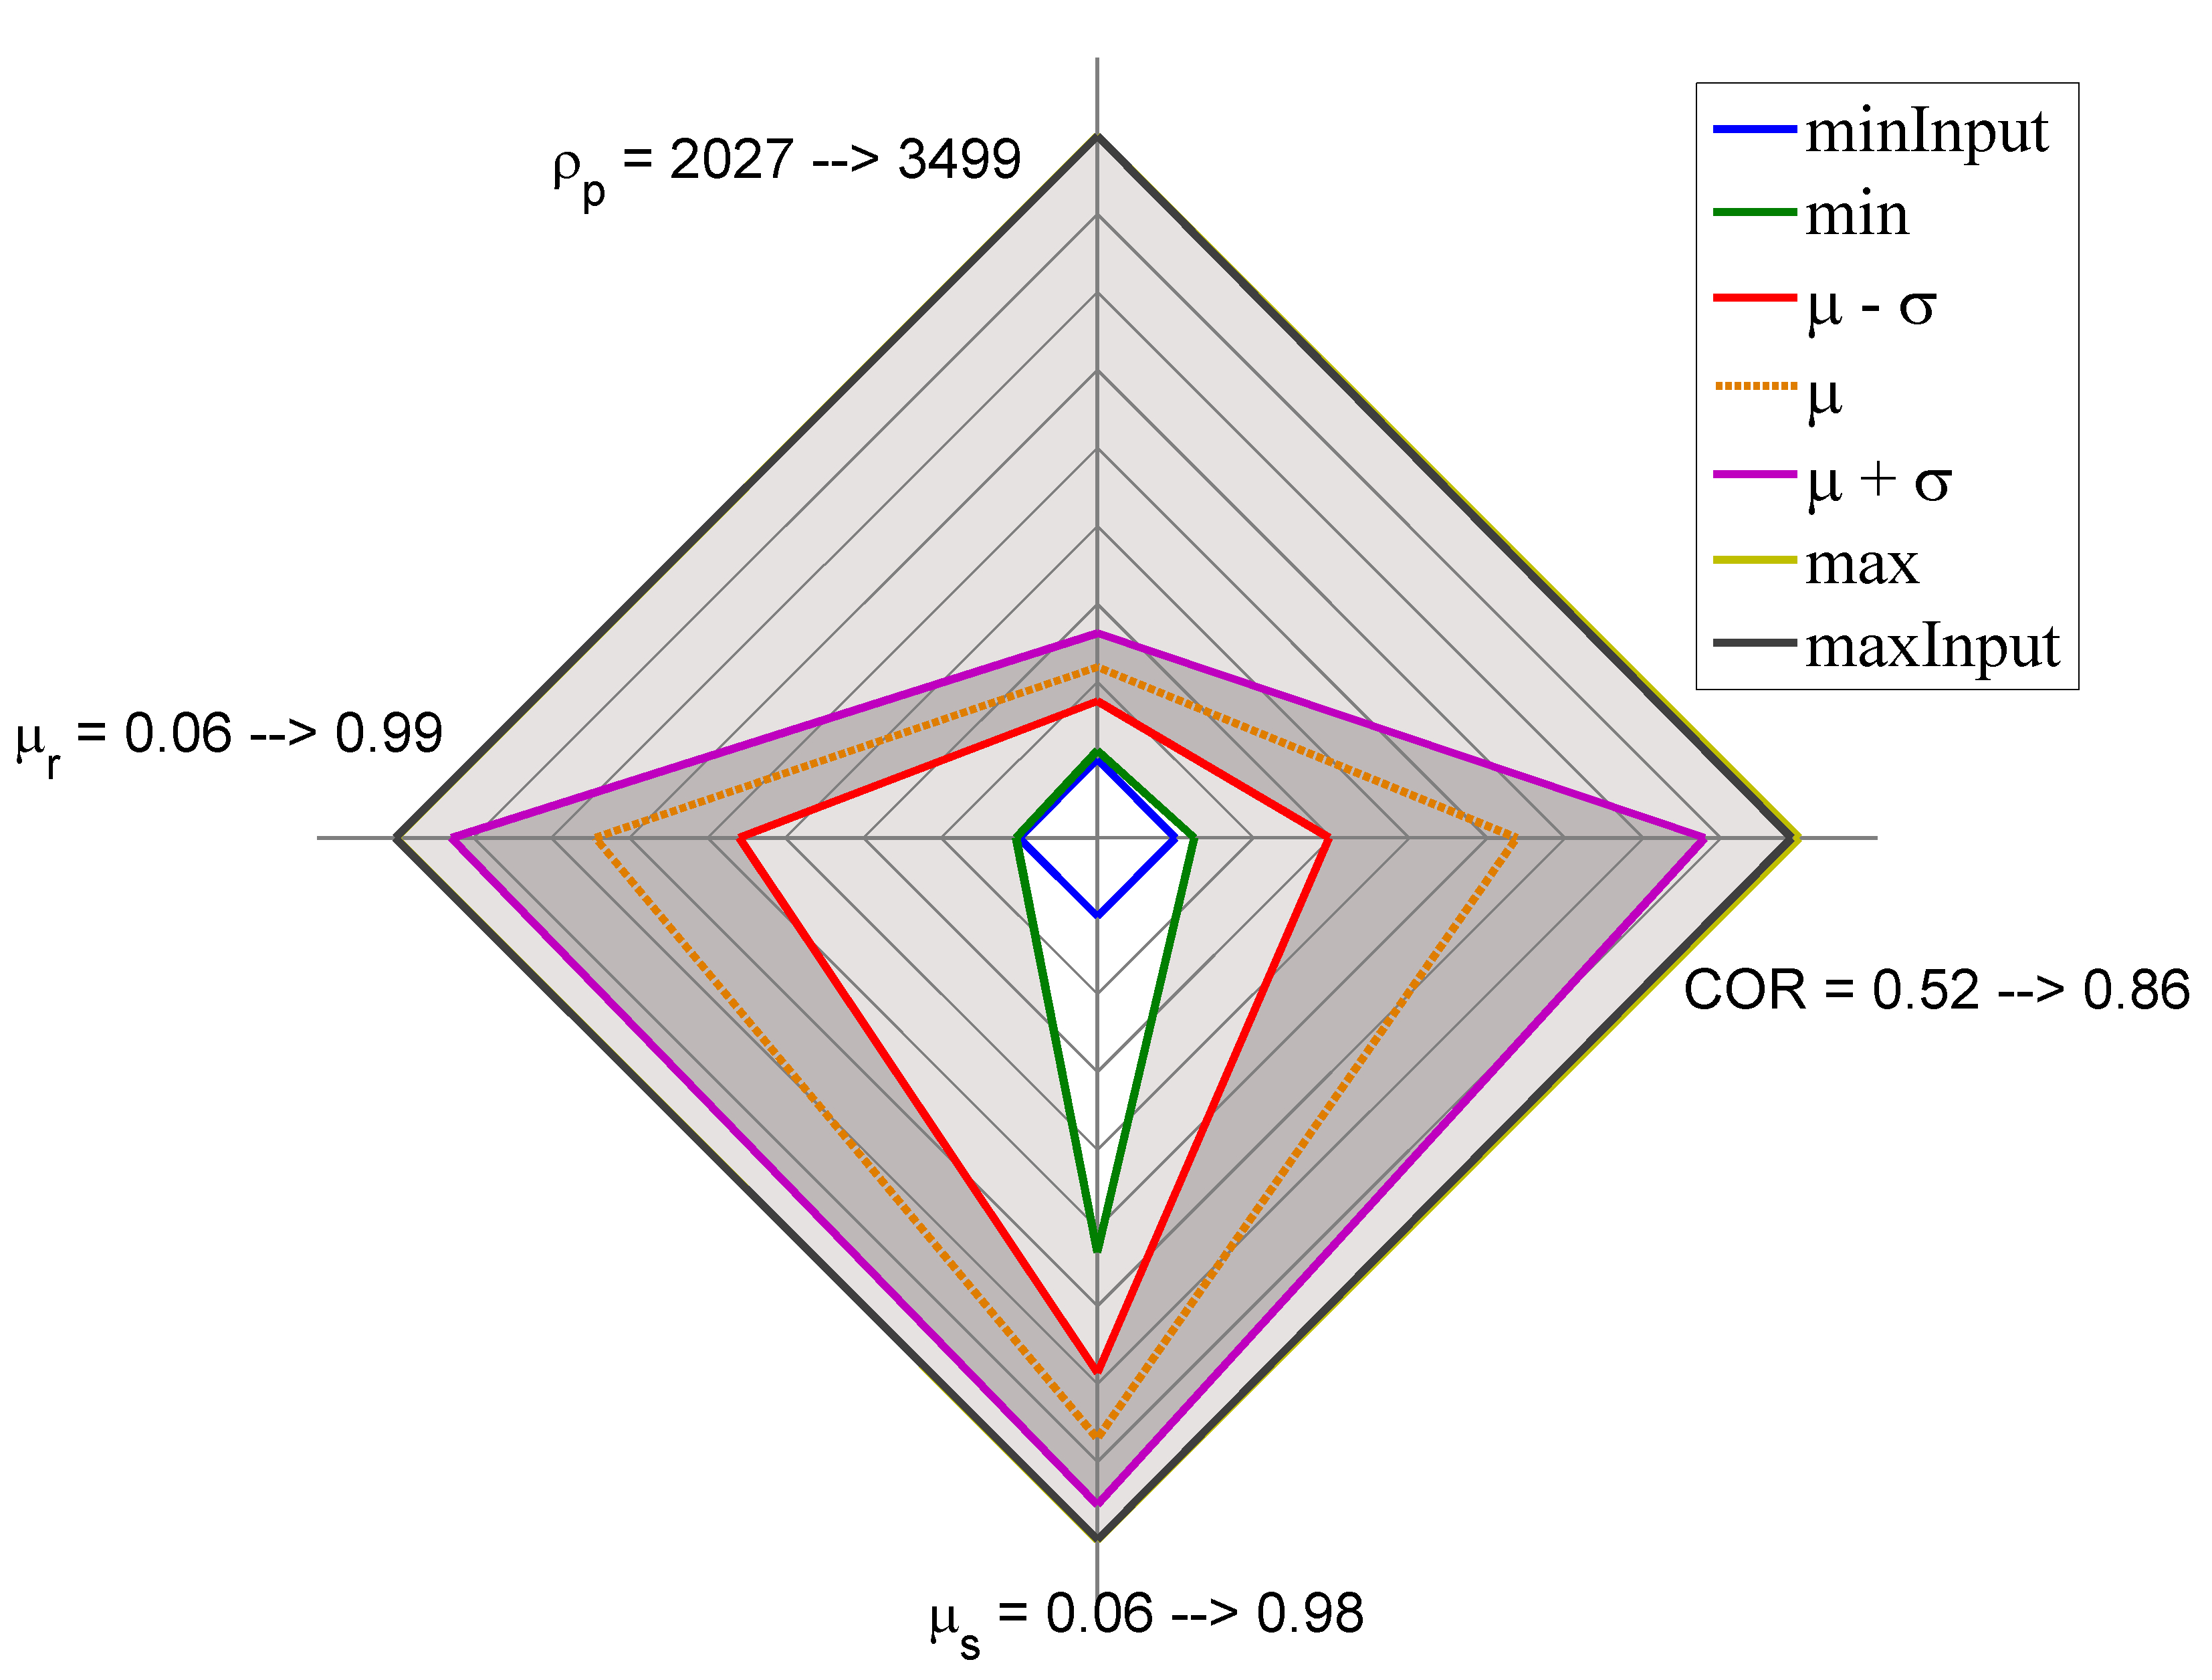
\includegraphics[width=.45\columnwidth]{images/original/24radarpirker1schulze10070}} \quad
\subfloat[Radar Schulze 10070 Pa and AOR]
{\label{fig:33radarpirker1schulze10070aor}%
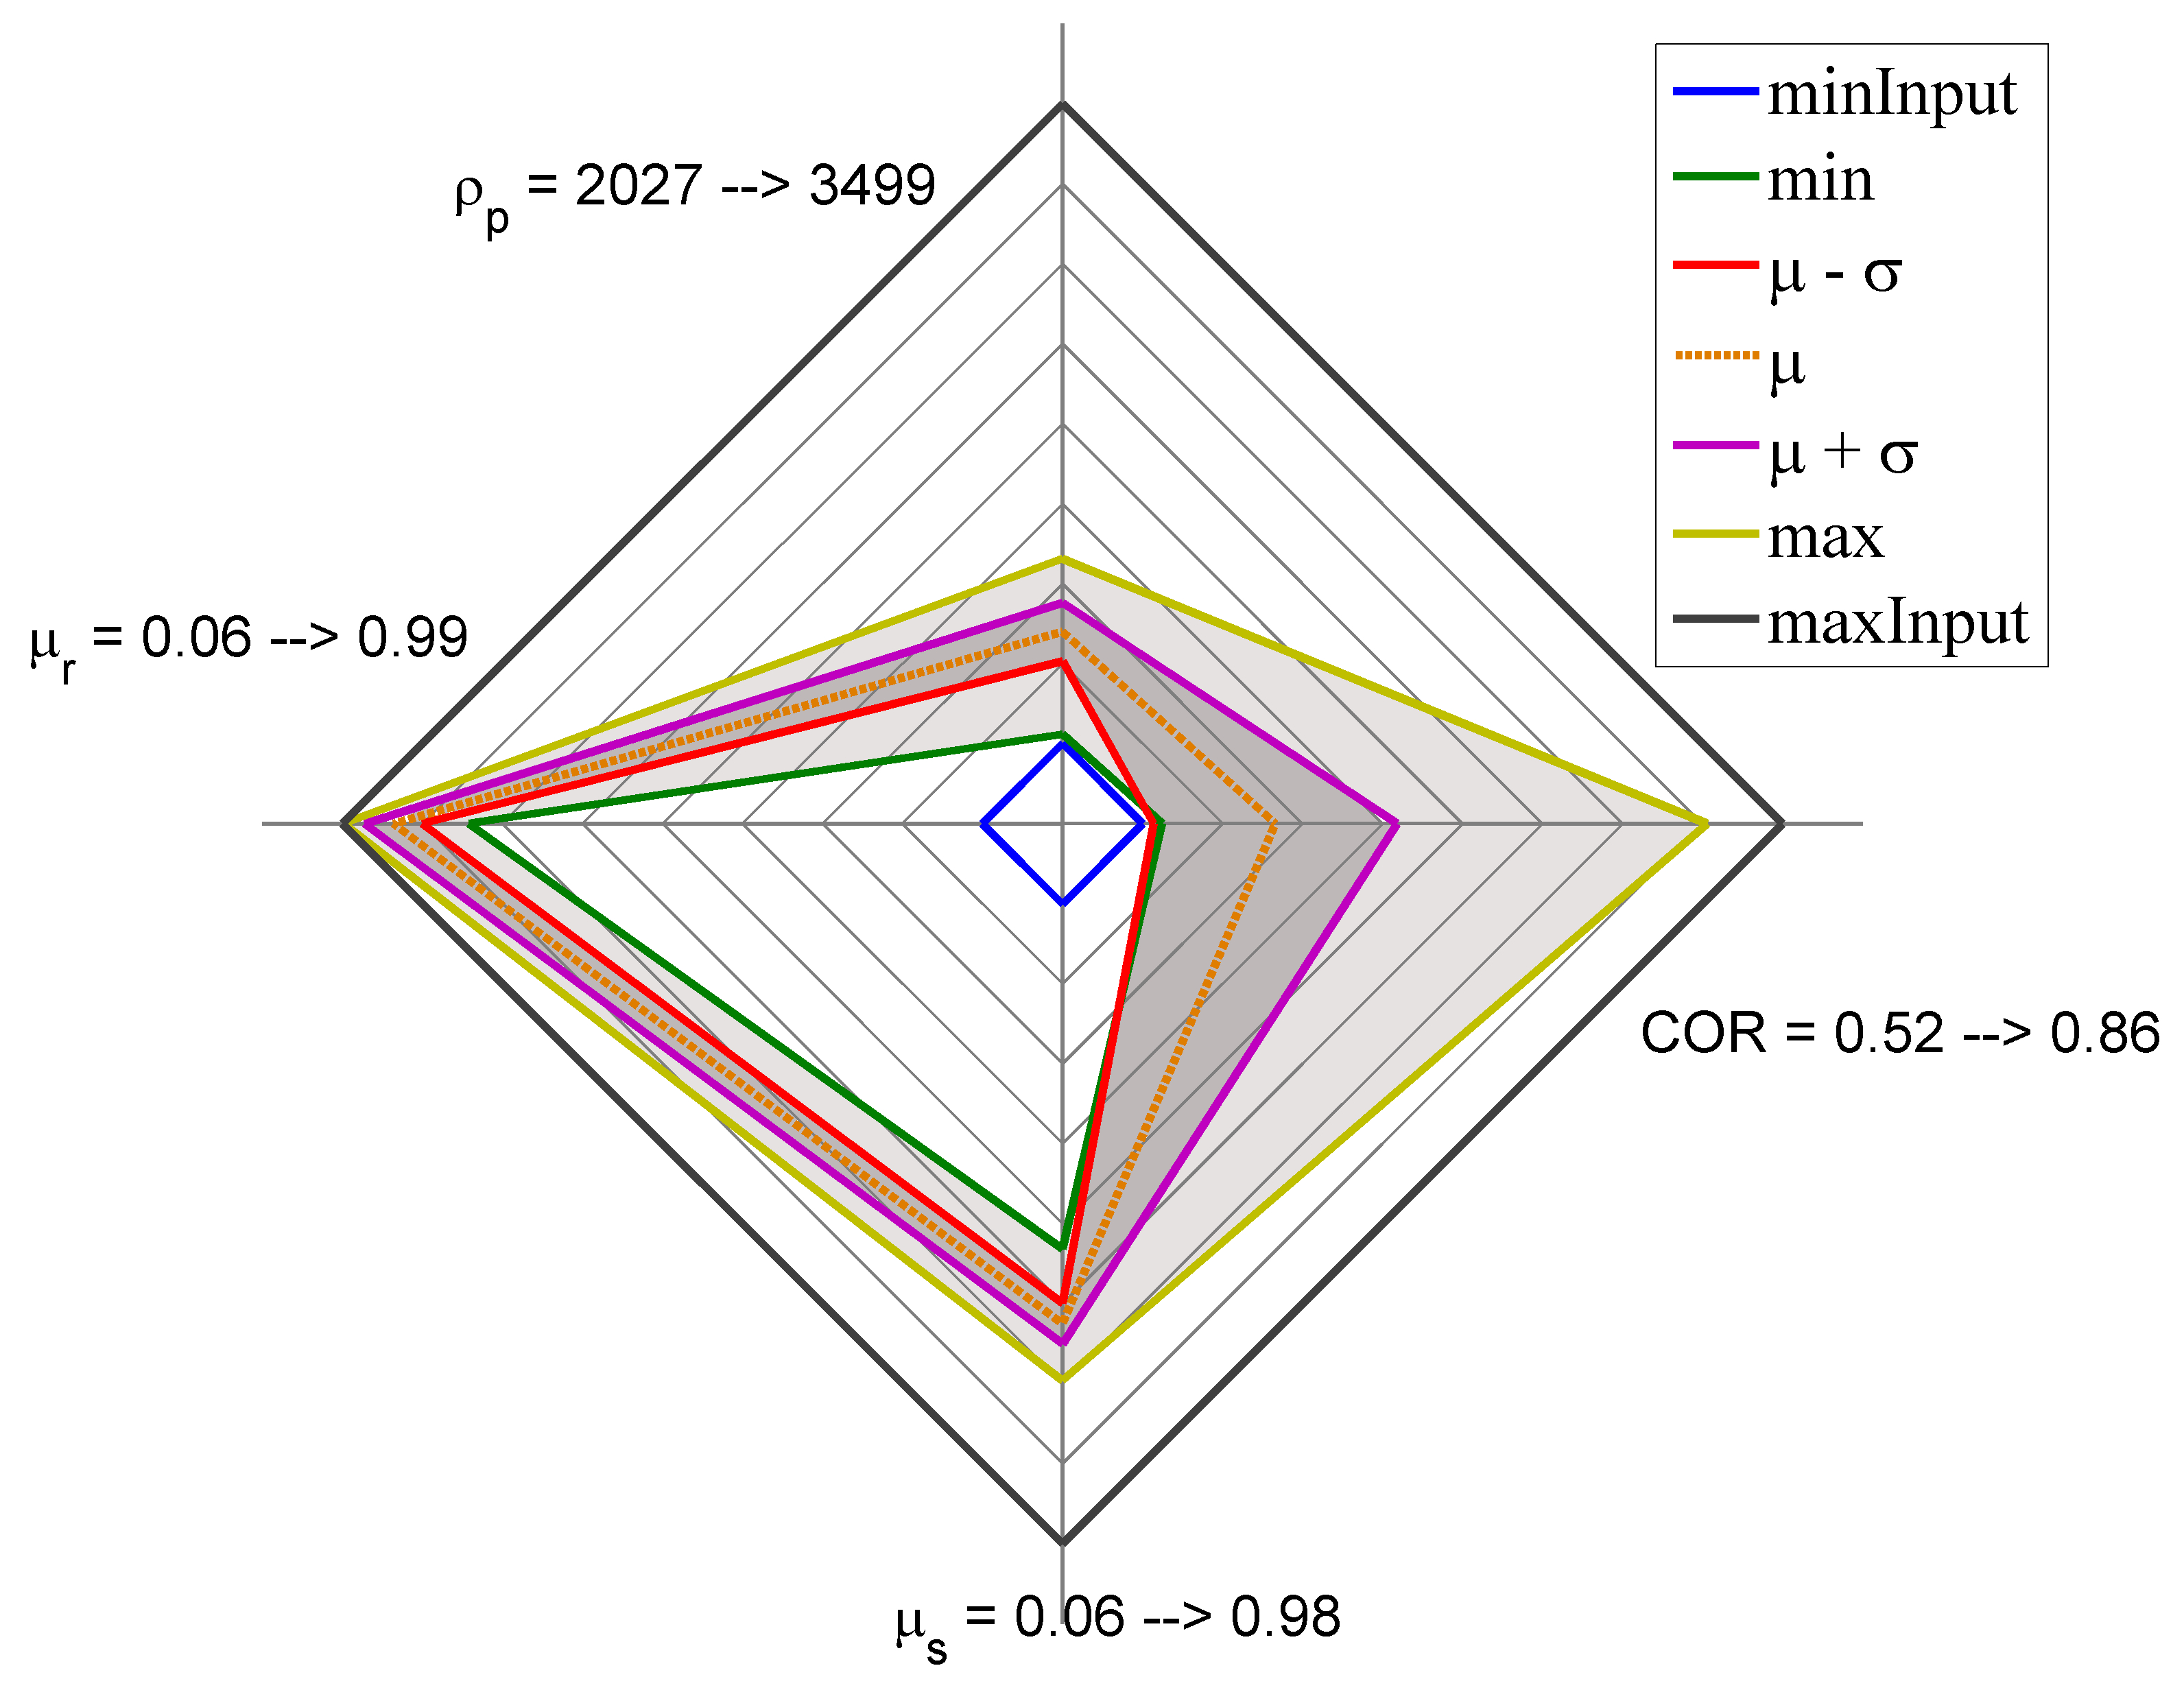
\includegraphics[width=.45\columnwidth]{images/original/33radarpirker1schulze10070aor}} \\
 \caption{Radar plots}
\label{fig:41schulze10070aor}
\end{figure}
